\documentclass[11pt]{article}
\usepackage[utf8]{inputenc}
\usepackage[spanish,es-tabla,es-nodecimaldot]{babel}

% Paquetess

\usepackage{amsmath}
\usepackage{amsthm}
\usepackage{amsfonts}
\usepackage{amssymb}
\usepackage{makeidx}
\usepackage{graphicx}
\usepackage{lmodern}
\usepackage[dvipsnames]{xcolor} 
\usepackage{fancyhdr}
\usepackage{geometry}
\usepackage{lastpage}		
\usepackage{array}			 % Para fjar tamaño de columnas
\usepackage{tikz}
\usepackage{subcaption}
\usepackage{caption}
\usepackage{pgfplots} % Para controlar la perspectiva
\RequirePackage{siunitx}
\usepackage{extramarks} % Para poder usar firstleftmarks
\usepackage[version=4]{mhchem} % Para poder usar formulas de reacciones nucleares
\usepackage{chemfig}
\usepackage{xcolor}
\RequirePackage[most]{tcolorbox}
\usepackage{enumitem}
\usepackage{physics}
%\usepackage{background}
\usepackage{eso-pic} % Para insertar imágenes de fondo específicas
\usepackage[absolute,overlay]{textpos} % Paquete para colocar elementos en posiciones absolutas
\usepackage{wrapfig}
\usepackage{booktabs}
\usepackage{float} % en el preámbulo

\setlength{\parindent}{0pt} % Elimina la sangría
\newtcolorbox{mybox}{colback=black!5!white,
	colframe=black!75!black}

\newtcolorbox{Anotacion}{colback=red!5!white,
	colframe=red!75!red}


%##############################################################################
%######### Ponemos el decimal con . ###########################################
%##############################################################################

\sisetup{output-decimal-marker={.},
	% exponentes ------------------------
	exponent-mode=threshold,
	exponent-thresholds=-3:4, % non usar exponentes 10^{-2,-1, 0, 1,2,3}
	% redondear -------------------------
	% round-mode=figures, % cifras sig
	% round-mode=places, % cantos decimales
	round-mode=uncertainty, % cifras sig da incerteza (necesario usar erro)
	round-precision=2,
	%uncertainty-mode = separate,
	print-unity-mantissa=false,
	% unidades --------------------------
	inter-unit-product = \ensuremath{{}\cdot{}}, % separacion entre unidades
	% per-mode=power-positive-first, % so furrula con metodo interpretado puro
	inline-per-mode=single-symbol,
	display-per-mode=fraction,
}

%##############################################################################
%######### Para codigo python #################################################
%##############################################################################

\definecolor{codegreen}{rgb}{0,0.6,0}
\definecolor{codegray}{rgb}{0.5,0.5,0.5}
\definecolor{codepurple}{rgb}{0.58,0,0.82}

\usepackage{listings}


%\lstdefinestyle{mystyle}{	backgroundcolor=\color{backcolour},   	commentstyle=\color{codegreen},	keywordstyle=\color{magenta},	numberstyle=\tiny\color{codegray},	stringstyle=\color{codepurple},	basicstyle=\ttfamily\footnotesize,	breakatwhitespace=false,         	breaklines=true,                 	captionpos=b,                    	keepspaces=true,                 	numbers=left,                    	numbersep=5pt,                  	showspaces=false,                	showstringspaces=false,	showtabs=false,                  	tabsize=2}

%\lstset{style=mystyle}
%\usepackage{background}     % Para manejar el fondo

%%%%%%%%%%%%%%%%%%%%%%%%%%%%%%%%%%%%%%%%%%
%%%%%%%%%%%%%%%%%% BIBLIOGRAFIA %%%%%%%%%%
%%%%%%%%%%%%%%%%%%%%%%%%%%%%%%%%%%%%%%%%%%


\usepackage{biblatex} %Imports biblatex package
\addbibresource{sample.bib} %Import the bibliography file

%##############################################################################
%######### Tipo de fuente #################################################
%##############################################################################

\usepackage{newtxtext,newtxmath} % Cambia la fuente (pero mola)
%\usepackage{kpfonts}

%\usepackage{helvet} 
%\renewcommand{\familydefault}{\sfdefault}.

%\usepackage{fontspec} % Paquete necesario para seleccionar fuentes
%\setmainfont{Verdana} % Cambia la fuente principal a Verdana


%##############################################################################
%######### Geometría #################################################
%##############################################################################

\geometry{a4paper, total={165mm,237mm}, left=22mm, top=30mm}



%##############################################################################
%######### Formatos capítulo #################################################
%##############################################################################

%\usepackage[lmodern]{quotchap}
%\usepackage[options]{fncychap}
% Configuración de la imagen de fondo solo para la portada



%##############################################################################
%######### Hiperreferenias #################################################
%##############################################################################


\usepackage[colorlinks=true, linkcolor=RoyalBlue, citecolor=ForestGreen, urlcolor=BrickRed]{hyperref} % Crea las
\usepackage[nameinlink]{cleveref}
\crefname{figure}{fig.}{Figs.}

%##############################################################################
%######### Formato de pagina #################################################
%##############################################################################

\pagestyle{fancy}
\fancyhf{} % Limpia encabezados y pies
\fancyhead[L]{\small \textbf{Memoria Rayos Cósmicos Analógicos}}    % Encabezado izquierdo
\fancyhead[R]{\small \textbf{Daniel Vázquez Lago}}     % Encabezado derecho
\fancyfoot[C]{\thepage}      % Pie de página centrado con el número de página
\renewcommand{\headrulewidth}{0.4pt}  % Grosor de la línea del encabezado
\renewcommand{\footrulewidth}{0pt}    % Sin línea en el pie



%##############################################################################
%#########  Modificar caption #################################################
%##############################################################################

\usepackage[font=small, justification=centering]{caption}  % Configura las captions



%##############################################################################
%######### Comandos propios #################################################
%##############################################################################


\newcommand{\parentesis}[1]{\left( #1  \right)}
\newcommand{\parciales}[2]{\frac{\partial #1}{\partial #2}}
\newcommand{\pparciales}[2]{\parentesis{\parciales{#1}{#2}}}
\newcommand{\ccorchetes}[1]{\left[ #1  \right]}
\newcommand{\D}{\mathrm{d}}
\newcommand{\derivadas}[2]{\frac{\D #1}{\D #2}}

\newcommand{\tquad}{\quad \quad \quad}
%\newcommand{\vnabla}{\vec{\nabla}}

\newcommand{\Ocal}{\mathcal{O}}
\newcommand{\Jcal}{\mathcal{J}}
\newcommand{\Mcal}{\mathcal{M}}
\newcommand{\Fcal}{\mathcal{F}}
\newcommand{\Hcal}{\mathcal{H}}
\newcommand{\Ecal}{\mathcal{E}}
\newcommand{\Ncal}{\mathcal{N}}

\newcommand{\cmm}{\text{cm}^{-1}}
\newcommand{\fcc}{\textit{fcc}}
\newcommand{\bcc}{\textit{bcc}}
\renewcommand{\sc}{\textit{sc}}
\newcommand{\hcp}{\textit{hcp}}


\newcommand{\PZB}{\text{{\tiny PZB}}}
\newcommand{\gap}{\text{{\tiny gap}}}
\newcommand{\SZB}{\text{{\tiny SZB}}}
\newcommand{\inicial}{\text{{\tiny inicial}}}
\newcommand{\final}{\text{{\tiny final}}}
\newcommand{\atomico}{\text{{\tiny atómico}}}

\newcommand{\arctanh}{\text{{arctanh}}}



\newcommand{\Namas}{\text{Na}^+}
\newcommand{\Clmenos}{\text{Cl}^-}

\newcommand{\cm}{\text{cm}}
\newcommand{\eV}{\text{eV}}

\newcommand{\arr}{\text{arr}}
\newcommand{\diff}{\text{diff}}

\newcommand{\er}{$^{\text{er}}$}
\newcommand{\cte}{\text{cte}}
\newcommand{\expo}{\text{exp}}
\newcommand{\simu}{\text{sim}}


% Comandos vectoriales

\newcommand{\an}{\mathbf{a}}
\newcommand{\bn}{\mathbf{b}}
\newcommand{\dn}{\mathbf{d}}
\newcommand{\fn}{\mathbf{f}}
\newcommand{\jn}{\mathbf{j}}
\newcommand{\kn}{\mathbf{k}}
\newcommand{\pn}{\mathbf{p}}
\newcommand{\qn}{\mathbf{q}}
\newcommand{\rn}{\mathbf{r}}
\newcommand{\sn}{\mathbf{s}}
\newcommand{\un}{\mathbf{u}}
\newcommand{\vn}{\mathbf{v}}
\newcommand{\xn}{\mathbf{x}}
\newcommand{\wn}{\mathbf{w}}
\newcommand{\yn}{\mathbf{y}}
\newcommand{\qndot}{\dot{\qn}}

\newcommand{\alphan}{\boldsymbol{\alpha}}
\newcommand{\sigman}{\boldsymbol{\sigma}}
\newcommand{\pin}{\boldsymbol{\pi}}
\newcommand{\rhon}{\boldsymbol{\rho}}
\newcommand{\epsilonn}{\boldsymbol{\epsilon}}
\newcommand{\omegan}{\boldsymbol{\omega}}
\newcommand{\mun}{\boldsymbol{\mu}}



\newcommand{\An}{\mathbf{A}}
\newcommand{\Bn}{\mathbf{B}}
\newcommand{\En}{\mathbf{E}}
\newcommand{\Fn}{\mathbf{F}}
\newcommand{\Jn}{\mathbf{J}}
\newcommand{\Hn}{\mathbf{H}}
\newcommand{\Gn}{\mathbf{G}}
\newcommand{\Kn}{\mathbf{K}}
\newcommand{\Ln}{\mathbf{L}}
\newcommand{\Mn}{\mathbf{M}}
\newcommand{\Pn}{\mathbf{P}}
%\newcommand{\Rn}{\mathbf{R}}
\newcommand{\Sn}{\mathbf{S}}
\newcommand{\Tn}{\mathbf{T}}
\newcommand{\In}{\mathbf{1}}
\newcommand{\Encal}{\boldsymbol{\mathcal{E}}}

\newcommand{\hnn}{\hat{\mathbf{n}}}
\newcommand{\hnr}{\hat{\mathbf{r}}}
\newcommand{\hnz}{\hat{\mathbf{z}}}
\newcommand{\hnv}{\hat{\mathbf{v}}}
\newcommand{\hnx}{\hat{\mathbf{x}}}
\newcommand{\hny}{\hat{\mathbf{y}}}
\newcommand{\hnu}{\hat{\mathbf{u}}}
\newcommand{\hnR}{\hat{\mathbf{R}}}
\newcommand{\hnp}{\hat{\mathbf{p}}}
\newcommand{\hnk}{\hat{\mathbf{k}}}
\newcommand{\hni}{\hat{\mathbf{i}}}
\newcommand{\hnj}{\hat{\mathbf{j}}}
\renewcommand{\hnk}{\hat{\mathbf{k}}}

 
\title{\textbf{\Huge Cósmicos Analógicos}}
\author{Daniel Vázquez Lago}
\date{\today}
\begin{document}
\maketitle
\newpage 
\tableofcontents
\newpage

\section{Objetivos}

Los objetivos basicamente son rascarme los huevos con \cite{Estadistica}.

\section{Caracterización de los detectores}


\subsection{Determinación de la ventana temporal}

\begin{center}
\begin{table}[H]
\caption{Ventana de coincidencias}
\label{Tab:ventana_01}
\begin{tabular}{cccccccccccccccccccccc}
\toprule
$N_1$ & $N_2$ & $N_{12}$ & $t$ (s) & $n_1$ (s$^{-1}$) & $n_2$ (s$^{-1}$) & $n_{12}$ (s$^{-1}$) & $\tau$ ($\mu$s) \\
\midrule
\num{45323.0000000000(212.8919913947)} & \num{10854.0000000000(104.1825321251)} & \num{154.0000000000(12.4096736460)} & \num{94.2100000000(0.3000000000)} & \num{481.0848105297(2.7300916193)} & \num{115.2106995011(1.1651224443)} & \num{1.6346460036(0.1318263382)} & \num{14.7461709041(1.2014395137)} \\
\num{84902.0000000000(291.3794776576)} & \num{21458.0000000000(146.4854941624)} & \num{268.0000000000(16.3707055437)} & \num{184.6800000000(0.3000000000)} & \num{459.7249296080(1.7455667243)} & \num{116.1901667750(0.8153325141)} & \num{1.4511587611(0.0886749683)} & \num{13.5836818887(0.8370943900)} \\
\num{48572.0000000000(220.3905624114)} & \num{21615.0000000000(147.0204067468)} & \num{103.0000000000(10.1488915651)} & \num{98.1000000000(0.3000000000)} & \num{495.1274209990(2.7092109749)} & \num{220.3363914373(1.6431861470)} & \num{1.0499490316(0.1035043668)} & \num{4.8121040597(0.4764626054)} \\
\num{43165.0000000000(207.7618829333)} & \num{16088.0000000000(126.8384799657)} & \num{181.0000000000(13.4536240471)} & \num{101.7400000000(0.3000000000)} & \num{424.2677413014(2.3948291109)} & \num{158.1285630037(1.3310341506)} & \num{1.7790446236(0.1323393577)} & \num{13.2588699141(0.9954110424)} \\
\bottomrule
\end{tabular}
\end{table}
\end{center}


\subsection{Determinación de la zona de trabajo}

\begin{center}
\begin{table}[H]
\caption{Medidas fijando el voltaje umbral}
\label{Tab:plateu_U}
\begin{tabular}{cccccccccccccccccccccc}
\toprule
$U_1$ (V) & $N_1$ & $N_2$ & $N_{12}$ & $t$ (s) & $n_1$ (s$^{-1}$) & $n_2$ (s$^{-1}$) & $n_{12}$ (s$^{-1}$) \\
\midrule
\num{-0.0590000000(0.0100000000)} & \num{1822.0000000000(42.6848919408)} & \num{40815.0000000000(202.0272258880)} & \num{350.0000000000(18.7082869339)} & \num{15.5000000000(0.3000000000)} & \num{117.5483870968(3.5721119464)} & \num{2633.2258064516(52.6059323045)} & \num{22.5806451613(1.2836759428)} \\
\num{-0.1000000000(0.0100000000)} & \num{9944.0000000000(99.7196068985)} & \num{3040.0000000000(55.1361950084)} & \num{223.0000000000(14.9331845231)} & \num{29.7200000000(0.3000000000)} & \num{334.5895020188(4.7607781038)} & \num{102.2880215343(2.1231615365)} & \num{7.5033647376(0.5081389212)} \\
\num{-0.3140000000(0.0100000000)} & \num{3764.0000000000(61.3514466007)} & \num{6482.0000000000(80.5108688315)} & \num{318.0000000000(17.8325545001)} & \num{51.4500000000(0.3000000000)} & \num{73.1584062196(1.2664526335)} & \num{125.9863945578(1.7286913207)} & \num{6.1807580175(0.3484683485)} \\
\num{-0.2090000000(0.0100000000)} & \num{6250.0000000000(79.0569415042)} & \num{5667.0000000000(75.2794792756)} & \num{323.0000000000(17.9722007556)} & \num{47.5200000000(0.3000000000)} & \num{131.5235690236(1.8593526864)} & \num{119.2550505051(1.7539650572)} & \num{6.7971380471(0.3806294656)} \\
\num{-0.4060000000(0.0100000000)} & \num{8208.0000000000(90.5980132232)} & \num{3060.0000000000(55.3172667438)} & \num{320.0000000000(17.8885438200)} & \num{66.5100000000(0.3000000000)} & \num{123.4100135318(1.4715207894)} & \num{46.0081190798(0.8572127469)} & \num{4.8113065704(0.2698343347)} \\
\bottomrule
\end{tabular}
\end{table}
\end{center}


\begin{center}
\begin{table}[H]
\caption{Medidas fijando el voltaje de ganancia}
\label{Tab:plateu_V}
\begin{tabular}{cccccccccccccccccccccc}
\toprule
$V_1$ (V) & $N_1$ & $N_2$ & $N_{12}$ & $t$ (s) & $n_1$ (s$^{-1}$) & $n_2$ (s$^{-1}$) & $n_{12}$ (s$^{-1}$) \\
\midrule
\num{1.4950000000(0.0100000000)} & \num{1026.0000000000(32.0312347561)} & \num{7436.0000000000(86.2322445492)} & \num{300.0000000000(17.3205080757)} & \num{65.2900000000(0.3000000000)} & \num{15.7145045183(0.4958845879)} & \num{113.8918670547(1.4206560605)} & \num{4.5948843621(0.2661245915)} \\
\num{1.7220000000(0.0100000000)} & \num{4737.0000000000(68.8258672303)} & \num{5695.0000000000(75.4652237789)} & \num{308.0000000000(17.5499287748)} & \num{48.9200000000(0.3000000000)} & \num{96.8315617334(1.5270897701)} & \num{116.4145543745(1.6998107824)} & \num{6.2959934587(0.3608192229)} \\
\num{1.8990000000(0.0100000000)} & \num{9944.0000000000(99.7196068985)} & \num{3040.0000000000(55.1361950084)} & \num{223.0000000000(14.9331845231)} & \num{29.7200000000(0.3000000000)} & \num{334.5895020188(4.7607781038)} & \num{102.2880215343(2.1231615365)} & \num{7.5033647376(0.5081389212)} \\
\num{1.9970000000(0.0100000000)} & \num{24917.0000000000(157.8511957509)} & \num{3904.0000000000(62.4819974073)} & \num{338.0000000000(18.3847763109)} & \num{33.7900000000(0.3000000000)} & \num{737.4075170169(8.0427679934)} & \num{115.5371411660(2.1145914584)} & \num{10.0029594555(0.5512897016)} \\
\bottomrule
\end{tabular}
\end{table}
\end{center}



\section{Caracterización estadística de la radiación cósmica secundaria}

\subsection{Numero de cuentas en 1 segundo}
\subsection{Numero de cuentas en 2 segundo}
\subsection{Numero de cuentas en 5 segundo}
\subsection{Numero de cuentas en 10 segundo}

\section{Atenuación de la radiación cósmica secundaria}

\subsection{Componente blanda}

\begin{center}
\begin{table}[H]
\caption{Medidas de atenuación blanda usando únicamente placas de hierro}
\label{Tab:hierro}
\begin{tabular}{cccccccccccccccccccccc}
\toprule
$x_{\text{Fe}}$ (mm) & $N_1$ & $N_2$ & $N_{12}$ & $t$ (s) & $n_1$ (s$^{-1}$) & $n_2$ (s$^{-1}$) & $n_{12}$ (s$^{-1}$) \\
\midrule
\num{0.0000000000(0.0000000000)} & \num{10319.0000000000(101.5824788042)} & \num{4468.0000000000(66.8430998683)} & \num{301.0000000000(17.3493515729)} & \num{41.1600000000(0.3000000000)} & \num{250.7045675413(3.0708263939)} & \num{108.5519922255(1.8064627215)} & \num{7.3129251701(0.4248666825)} \\
\num{0.0000000000(0.0000000000)} & \num{10326.0000000000(101.6169277237)} & \num{3988.0000000000(63.1506136154)} & \num{313.0000000000(17.6918060130)} & \num{36.6000000000(0.3000000000)} & \num{282.1311475410(3.6133627833)} & \num{108.9617486339(1.9428784119)} & \num{8.5519125683(0.4884388324)} \\
\num{0.0000000000(0.0000000000)} & \num{17115.0000000000(130.8243096676)} & \num{6221.0000000000(78.8733161468)} & \num{462.0000000000(21.4941852602)} & \num{52.5000000000(0.3000000000)} & \num{326.0000000000(3.1112313550)} & \num{118.4952380952(1.6478888775)} & \num{8.8000000000(0.4124896371)} \\
\num{3.2000000000(0.3200000000)} & \num{10973.0000000000(104.7520882847)} & \num{4699.0000000000(68.5492523665)} & \num{319.0000000000(17.8605710995)} & \num{46.1400000000(0.3000000000)} & \num{237.8196792371(2.7468753789)} & \num{101.8422193325(1.6265659460)} & \num{6.9137407889(0.3896965797)} \\
\num{3.2000000000(0.3200000000)} & \num{11183.0000000000(105.7497044913)} & \num{3966.0000000000(62.9761859753)} & \num{341.0000000000(18.4661853126)} & \num{39.0700000000(0.3000000000)} & \num{286.2298438700(3.4866178881)} & \num{101.5101100589(1.7904466319)} & \num{8.7279242385(0.4773712672)} \\
\num{3.2000000000(0.3200000000)} & \num{16251.0000000000(127.4794101022)} & \num{5668.0000000000(75.2861208989)} & \num{406.0000000000(20.1494416796)} & \num{51.4100000000(0.3000000000)} & \num{316.1058159891(3.0905231171)} & \num{110.2509239448(1.5995180421)} & \num{7.8972962459(0.3946362421)} \\
\num{6.4000000000(0.6400000000)} & \num{10263.0000000000(101.3064657364)} & \num{4357.0000000000(66.0075753228)} & \num{307.0000000000(17.5214154679)} & \num{43.9000000000(0.3000000000)} & \num{233.7813211845(2.8067103271)} & \num{99.2482915718(1.6494795990)} & \num{6.9931662870(0.4019719566)} \\
\num{6.4000000000(0.6400000000)} & \num{11621.0000000000(107.8007421125)} & \num{4059.0000000000(63.7102817448)} & \num{325.0000000000(18.0277563773)} & \num{41.4800000000(0.3000000000)} & \num{280.1591128255(3.2953993674)} & \num{97.8543876567(1.6911370874)} & \num{7.8351012536(0.4382918597)} \\
\num{6.4000000000(0.6400000000)} & \num{17252.0000000000(131.3468690148)} & \num{6003.0000000000(77.4790294209)} & \num{461.0000000000(21.4709105536)} & \num{54.5300000000(0.3000000000)} & \num{316.3763066202(2.9717730690)} & \num{110.0861910875(1.5445470175)} & \num{8.4540619842(0.3964823973)} \\
\num{6.4000000000(0.6400000000)} & \num{10593.0000000000(102.9223007905)} & \num{4296.0000000000(65.5438784327)} & \num{306.0000000000(17.4928556845)} & \num{43.6400000000(0.3000000000)} & \num{242.7360219982(2.8890656290)} & \num{98.4417965170(1.6473416901)} & \num{7.0119156737(0.4037324168)} \\
\num{9.6000000000(0.9600000000)} & \num{10886.0000000000(104.3359957062)} & \num{4153.0000000000(64.4437739429)} & \num{323.0000000000(17.9722007556)} & \num{45.5300000000(0.3000000000)} & \num{239.0951021305(2.7808810611)} & \num{91.2145837909(1.5377316149)} & \num{7.0942235888(0.3974912515)} \\
\num{9.6000000000(0.9600000000)} & \num{9617.0000000000(98.0663041008)} & \num{4161.0000000000(64.5058136915)} & \num{314.0000000000(17.7200451467)} & \num{39.8000000000(0.3000000000)} & \num{241.6331658291(3.0640693540)} & \num{104.5477386935(1.8021785981)} & \num{7.8894472362(0.4491812371)} \\
\num{9.6000000000(0.9600000000)} & \num{10291.0000000000(101.4445661433)} & \num{3659.0000000000(60.4896685393)} & \num{319.0000000000(17.8605710995)} & \num{53.3800000000(0.3000000000)} & \num{192.7875608842(2.1875876711)} & \num{68.5462720120(1.1968815897)} & \num{5.9760209816(0.3362743468)} \\
\num{9.6000000000(0.9600000000)} & \num{16542.0000000000(128.6157066614)} & \num{5511.0000000000(74.2361098119)} & \num{445.0000000000(21.0950231097)} & \num{37.5100000000(0.3000000000)} & \num{441.0023993602(4.9190662263)} & \num{146.9208211144(2.3016503089)} & \num{11.8635030658(0.5703318969)} \\
\num{12.8000000000(1.2800000000)} & \num{14495.0000000000(120.3951826279)} & \num{3481.0000000000(59.0000000000)} & \num{314.0000000000(17.7200451467)} & \num{37.4900000000(0.3000000000)} & \num{386.6364363830(4.4593020358)} & \num{92.8514270472(1.7403337905)} & \num{8.3755668178(0.4773887588)} \\
\num{12.8000000000(1.2800000000)} & \num{15148.0000000000(123.0772115381)} & \num{5310.0000000000(72.8697468089)} & \num{408.0000000000(20.1990098767)} & \num{53.3800000000(0.3000000000)} & \num{283.7766953915(2.8035161633)} & \num{99.4754589734(1.4751551304)} & \num{7.6433121019(0.3808307172)} \\
\num{16.0000000000(1.6000000000)} & \num{12982.0000000000(113.9385799455)} & \num{4297.0000000000(65.5515064663)} & \num{333.0000000000(18.2482875909)} & \num{46.1800000000(0.3000000000)} & \num{281.1173668255(3.0696148825)} & \num{93.0489389346(1.5428250929)} & \num{7.2109138155(0.3979225797)} \\
\num{16.0000000000(1.6000000000)} & \num{14880.0000000000(121.9836054558)} & \num{5181.0000000000(71.9791636517)} & \num{421.0000000000(20.5182845287)} & \num{54.3600000000(0.3000000000)} & \num{273.7306843267(2.7051053837)} & \num{95.3090507726(1.4247657066)} & \num{7.7446651950(0.3798640777)} \\
\num{19.2000000000(1.9200000000)} & \num{12682.0000000000(112.6143862923)} & \num{4502.0000000000(67.0969447889)} & \num{319.0000000000(17.8605710995)} & \num{50.8300000000(0.3000000000)} & \num{249.4983277592(2.6602399430)} & \num{88.5697422782(1.4197633433)} & \num{6.2758213653(0.3533254073)} \\
\num{19.2000000000(1.9200000000)} & \num{14553.0000000000(120.6358155773)} & \num{4987.0000000000(70.6186944088)} & \num{436.0000000000(20.8806130178)} & \num{52.3100000000(0.3000000000)} & \num{278.2068438157(2.8043063675)} & \num{95.3354999044(1.4565194433)} & \num{8.3349264003(0.4020225132)} \\
\num{19.2000000000(1.9200000000)} & \num{17022.0000000000(130.4683869755)} & \num{5593.0000000000(74.7863623932)} & \num{415.0000000000(20.3715487875)} & \num{55.7100000000(0.3000000000)} & \num{305.5465805062(2.8621422093)} & \num{100.3949021720(1.4471968371)} & \num{7.4492909711(0.3678650482)} \\
\num{22.4000000000(2.2400000000)} & \num{14875.0000000000(121.9631091765)} & \num{5291.0000000000(72.7392603757)} & \num{426.0000000000(20.6397674406)} & \num{54.0300000000(0.3000000000)} & \num{275.3100129558(2.7262201071)} & \num{97.9270775495(1.4519323911)} & \num{7.8845086063(0.3845060530)} \\
\num{22.4000000000(2.2400000000)} & \num{17365.0000000000(131.7763256431)} & \num{5844.0000000000(76.4460594145)} & \num{411.0000000000(20.2731349327)} & \num{58.0600000000(0.3000000000)} & \num{299.0871512229(2.7458366643)} & \num{100.6544953496(1.4156698615)} & \num{7.0788839132(0.3510861396)} \\
\num{25.6000000000(2.5600000000)} & \num{15848.0000000000(125.8888398548)} & \num{5617.0000000000(74.9466476902)} & \num{417.0000000000(20.4205778567)} & \num{57.8800000000(0.3000000000)} & \num{273.8078783690(2.5970552316)} & \num{97.0456116102(1.3891288373)} & \num{7.2045611610(0.3547795747)} \\
\num{28.8000000000(2.8800000000)} & \num{14736.0000000000(121.3919272439)} & \num{5358.0000000000(73.1983606374)} & \num{417.0000000000(20.4205778567)} & \num{53.9300000000(0.3000000000)} & \num{273.2430928982(2.7160609779)} & \num{99.3510105693(1.4654903037)} & \num{7.7322455034(0.3810848713)} \\
\num{28.8000000000(2.8800000000)} & \num{17707.0000000000(133.0676519670)} & \num{5842.0000000000(76.4329771761)} & \num{413.0000000000(20.3224014329)} & \num{61.2600000000(0.3000000000)} & \num{289.0466862553(2.5926861493)} & \num{95.3640222005(1.3322201264)} & \num{6.7417564479(0.3333789824)} \\
\num{32.0000000000(3.2000000000)} & \num{16089.0000000000(126.8424219258)} & \num{5557.0000000000(74.5452882482)} & \num{415.0000000000(20.3715487875)} & \num{58.8400000000(0.3000000000)} & \num{273.4364377974(2.5672420945)} & \num{94.4425560843(1.3553367372)} & \num{7.0530251530(0.3480819042)} \\
\num{32.0000000000(3.2000000000)} & \num{16089.0000000000(126.8424219258)} & \num{5557.0000000000(74.5452882482)} & \num{415.0000000000(20.3715487875)} & \num{58.8400000000(0.3000000000)} & \num{273.4364377974(2.5672420945)} & \num{94.4425560843(1.3553367372)} & \num{7.0530251530(0.3480819042)} \\
\bottomrule
\end{tabular}
\end{table}
\end{center}


\begin{figure} \centering
    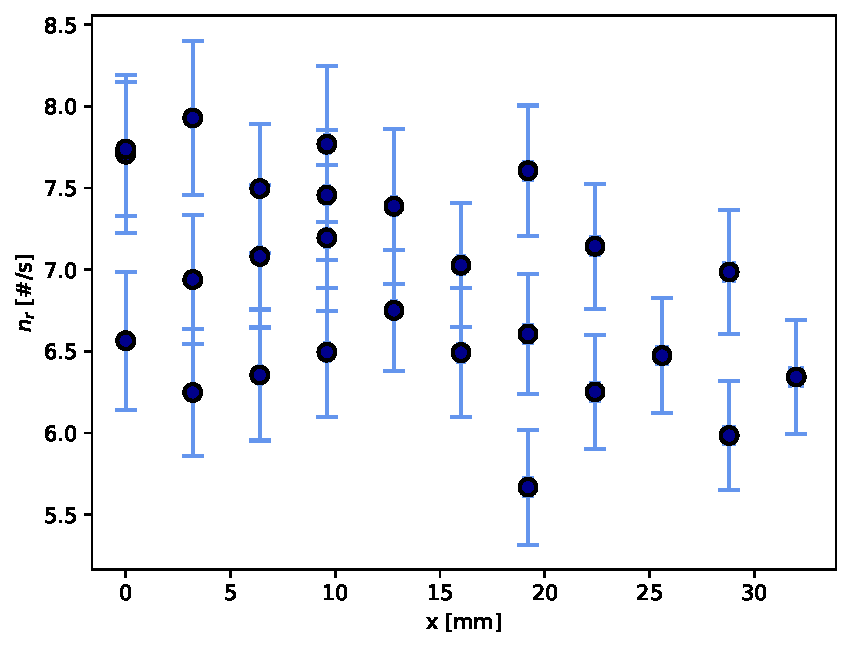
\includegraphics[width=0.5\linewidth]{../Graficas/Atenuacion_Fe.pdf}
\end{figure}

\subsection{Componente blanda y dura}


\begin{center}
\begin{table}[H]
\caption{Medidas de atenuación dura usando únicamente placas de plomo con 20 de hierro}
\small
\label{Tab:plomo_1}
\begin{tabular}{cccccccccccccccccccccc}
\toprule
$x_{\text{Pb}}$ (mm) & $N_1$  & $N_2$ & $N_{12}$ & $t$ [s] & $n_1$ [s$^{-1}$] & $n_2$  [s$^{-1}$] & $n_{acc}$ [s$^{-1}$] & $n_{r}$ [s$^{-1}$] \\
\midrule
\num{0.0(0.0)} & \num{16089.0000000000(126.8424219258)} & \num{5557.0000000000(74.5452882482)} & \num{415.0000000000(20.3715487875)} & \num{58.8400000000(0.1300000000)} & \num{273.4364377974(2.2387687945)} & \num{94.4425560843(1.2839832053)} & \num{0.7096445124(0.0157600682)} & \num{6.3433806406(0.3469280454)} \\
\num{0.0(0.0)} & \num{16089.0000000000(126.8424219258)} & \num{5557.0000000000(74.5452882482)} & \num{415.0000000000(20.3715487875)} & \num{58.8400000000(0.1300000000)} & \num{273.4364377974(2.2387687945)} & \num{94.4425560843(1.2839832053)} & \num{0.7096445124(0.0157600682)} & \num{6.3433806406(0.3469280454)} \\
\num{7.5000000000(0.0140000000)} & \num{17091.0000000000(130.7325514170)} & \num{5418.0000000000(73.6070648783)} & \num{406.0000000000(20.1494416796)} & \num{62.2200000000(0.1300000000)} & \num{274.6865959499(2.1781062908)} & \num{87.0781099325(1.1969214170)} & \num{0.6572993302(0.0145973470)} & \num{5.8679337139(0.3244572681)} \\
\num{7.5000000000(0.0140000000)} & \num{16888.0000000000(129.9538379579)} & \num{5633.0000000000(75.0533143838)} & \num{412.0000000000(20.2977831302)} & \num{60.6600000000(0.1300000000)} & \num{278.4042202440(2.2238640690)} & \num{92.8618529509(1.2531814349)} & \num{0.7104440608(0.0157540322)} & \num{6.0815110991(0.3353023553)} \\
\num{15.0000000000(0.0280000000)} & \num{17940.0000000000(133.9402852020)} & \num{5424.0000000000(73.6478105581)} & \num{409.0000000000(20.2237484162)} & \num{65.3100000000(0.1300000000)} & \num{274.6899402848(2.1224749278)} & \num{83.0500689022(1.1397177916)} & \num{0.6269017475(0.0139089319)} & \num{5.6355389201(0.3102205260)} \\
\num{15.0000000000(0.0280000000)} & \num{18321.0000000000(135.3550885634)} & \num{6061.0000000000(77.8524244966)} & \num{415.0000000000(20.3715487875)} & \num{67.1300000000(0.1300000000)} & \num{272.9182183822(2.0844300167)} & \num{90.2875018621(1.1728324490)} & \num{0.6771375421(0.0149433283)} & \num{5.5048973157(0.3040676243)} \\
\num{15.0000000000(0.0280000000)} & \num{18008.0000000000(134.1938895777)} & \num{5570.0000000000(74.6324326282)} & \num{406.0000000000(20.1494416796)} & \num{64.8600000000(0.1300000000)} & \num{277.6441566451(2.1425093081)} & \num{85.8772741289(1.1634722706)} & \num{0.6552145257(0.0145188810)} & \num{5.6044216137(0.3112525815)} \\
\num{22.5000000000(0.0420000000)} & \num{16645.0000000000(129.0155029444)} & \num{5288.0000000000(72.7186358508)} & \num{414.0000000000(20.3469899494)} & \num{62.5000000000(0.1300000000)} & \num{266.3200000000(2.1372823229)} & \num{84.6080000000(1.1767321673)} & \num{0.6192014143(0.0137722560)} & \num{6.0047985857(0.3261341842)} \\
\num{37.5000000000(0.0700000000)} & \num{17336.0000000000(131.6662447251)} & \num{5496.0000000000(74.1350119714)} & \num{408.0000000000(20.1990098767)} & \num{66.0000000000(0.1300000000)} & \num{262.6666666667(2.0609399710)} & \num{83.2727272727(1.1351701274)} & \num{0.6010692073(0.0133336302)} & \num{5.5807489745(0.3065778205)} \\
\num{45.0000000000(0.0840000000)} & \num{17645.0000000000(132.8344834747)} & \num{5710.0000000000(75.5645419493)} & \num{405.0000000000(20.1246117975)} & \num{66.6600000000(0.1300000000)} & \num{264.7014701470(2.0584950096)} & \num{85.6585658566(1.1458241552)} & \num{0.6230800996(0.0137938480)} & \num{5.4525274611(0.3024465040)} \\
\num{52.5000000000(0.0980000000)} & \num{18037.0000000000(134.3018987208)} & \num{5662.0000000000(75.2462623656)} & \num{419.0000000000(20.4694894905)} & \num{67.5700000000(0.1300000000)} & \num{266.9379902324(2.0528746652)} & \num{83.7945833950(1.1252135167)} & \num{0.6146714772(0.0136078684)} & \num{5.5863052877(0.3034776059)} \\
\num{60.0000000000(0.1120000000)} & \num{18094.0000000000(134.5139397981)} & \num{5698.0000000000(75.4850978671)} & \num{410.0000000000(20.2484567313)} & \num{67.7400000000(0.1300000000)} & \num{267.1095364629(2.0508358765)} & \num{84.1157366401(1.1259673869)} & \num{0.6174238118(0.0136641717)} & \num{5.4351300707(0.2994518418)} \\
\num{67.5000000000(0.1260000000)} & \num{17038.0000000000(130.5296901092)} & \num{5252.0000000000(72.4706837280)} & \num{404.0000000000(20.0997512422)} & \num{63.4900000000(0.1300000000)} & \num{268.3572216097(2.1280721505)} & \num{82.7216884549(1.1539488288)} & \num{0.6100274890(0.0135669850)} & \num{5.7531793153(0.3171396927)} \\
\num{67.5000000000(0.1260000000)} & \num{18248.0000000000(135.0851583261)} & \num{5732.0000000000(75.7099729230)} & \num{416.0000000000(20.3960780544)} & \num{67.0600000000(0.1300000000)} & \num{272.1145243066(2.0823171813)} & \num{85.4756934089(1.1410835431)} & \num{0.6391622019(0.0141403620)} & \num{5.5642377385(0.3047126271)} \\
\num{75.0000000000(0.1400000000)} & \num{19374.0000000000(139.1905169184)} & \num{5953.0000000000(77.1556867638)} & \num{407.0000000000(20.1742410018)} & \num{72.1900000000(0.1300000000)} & \num{268.3751212079(1.9877605198)} & \num{82.4629450062(1.0790534669)} & \num{0.6081599586(0.0134177011)} & \num{5.0297400275(0.2799664040)} \\
\bottomrule
\end{tabular}
\end{table}
\end{center}


\begin{figure}[h!] \centering
    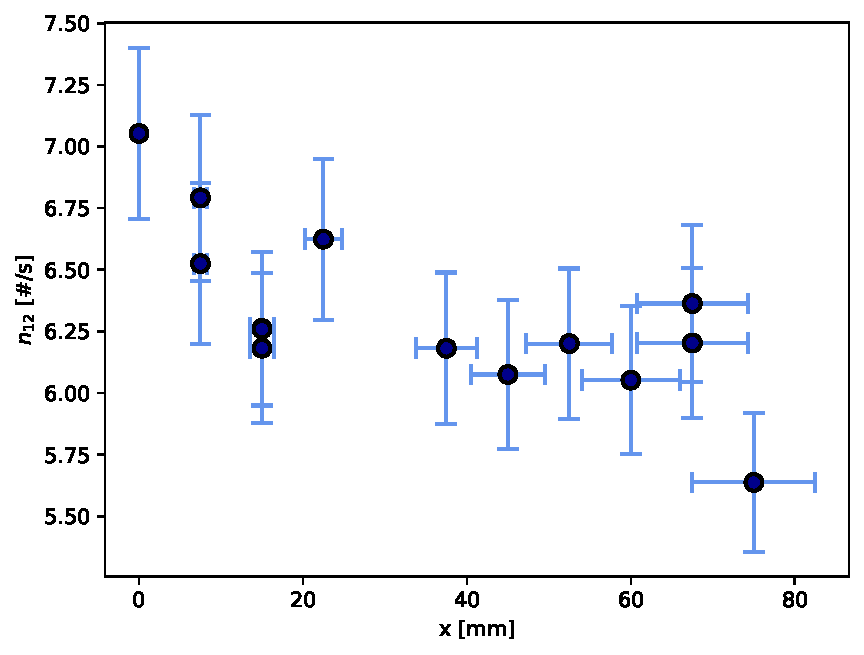
\includegraphics[width=0.5\linewidth]{../Graficas/Atenuacion_Pb.pdf}
\end{figure}


\subsection{Componente dura}

\begin{center}
\begin{table}[H]
\caption{Medidas de atenuación dura usando únicamente placas de plomo sin planchas de hierro}
\small
\label{Tab:plomo_2}
\begin{tabular}{cccccccccccccccccccccc}
\toprule
$x_{\text{Pb}}$ (mm) & $N_1$  & $N_2$ & $N_{12}$ & $t$ [s] & $n_1$ [s$^{-1}$] & $n_2$  [s$^{-1}$] & $n_{acc}$ [s$^{-1}$] & $n_{r}$ [s$^{-1}$] \\
\midrule
\num{0.0(0.0)} & \num{10326.0000000000(101.6169277237)} & \num{3988.0000000000(63.1506136154)} & \num{313.0000000000(17.6918060130)} & \num{36.6000000000(0.1300000000)} & \num{282.1311475410(2.9517310291)} & \num{108.9617486339(1.7682995938)} & \num{0.8447765074(0.0193277084)} & \num{7.7071360609(0.4847216248)} \\
\num{0.0(0.0)} & \num{17115.0000000000(130.8243096676)} & \num{6221.0000000000(78.8733161468)} & \num{462.0000000000(21.4941852602)} & \num{52.5000000000(0.1300000000)} & \num{326.0000000000(2.6193810628)} & \num{118.4952380952(1.5307336676)} & \num{1.0615372206(0.0234526395)} & \num{7.7384627794(0.4106627555)} \\
\num{7.5000000000(0.0140000000)} & \num{17450.0000000000(132.0984481362)} & \num{5952.0000000000(77.1492060879)} & \num{448.0000000000(21.1660104885)} & \num{61.6800000000(0.1300000000)} & \num{282.9118028534(2.2231321958)} & \num{96.4980544747(1.2672254112)} & \num{0.7502160517(0.0165863226)} & \num{6.5130783711(0.3438999098)} \\
\num{15.0000000000(0.0280000000)} & \num{16334.0000000000(127.8045382606)} & \num{5467.0000000000(73.9391641825)} & \num{429.0000000000(20.7123151772)} & \num{59.2600000000(0.1300000000)} & \num{275.6328045899(2.2398351409)} & \num{92.2544718191(1.2640145202)} & \num{0.6987712999(0.0155260323)} & \num{6.5405132090(0.3502208765)} \\
\num{22.5000000000(0.0420000000)} & \num{19751.0000000000(140.5382510209)} & \num{6151.0000000000(78.4283112148)} & \num{466.0000000000(21.5870331449)} & \num{77.3000000000(0.1300000000)} & \num{255.5109961190(1.8681796595)} & \num{79.5730918499(1.0233839183)} & \num{0.5587178630(0.0123039893)} & \num{5.4697426804(0.2797177548)} \\
\num{37.5000000000(0.0700000000)} & \num{18875.0000000000(137.3863166403)} & \num{5947.0000000000(77.1167945392)} & \num{413.0000000000(20.3224014329)} & \num{69.0000000000(0.1300000000)} & \num{273.5507246377(2.0567268633)} & \num{86.1884057971(1.1293696820)} & \num{0.6478932357(0.0143022089)} & \num{5.3376140107(0.2950901671)} \\
\num{52.5000000000(0.0980000000)} & \num{21546.0000000000(146.7855578727)} & \num{6703.0000000000(81.8718510845)} & \num{471.0000000000(21.7025344142)} & \num{78.0700000000(0.1300000000)} & \num{275.9830920968(1.9355276044)} & \num{85.8588446266(1.0583986971)} & \num{0.6511547974(0.0142739850)} & \num{5.3818924679(0.2785355961)} \\
\num{67.5000000000(0.1260000000)} & \num{18783.0000000000(137.0510853660)} & \num{5993.0000000000(77.4144689318)} & \num{444.0000000000(21.0713075057)} & \num{69.2600000000(0.1300000000)} & \num{271.1954952353(2.0432147453)} & \num{86.5290210800(1.1294752541)} & \num{0.6448533943(0.0142311445)} & \num{5.7657732300(0.3048051343)} \\
\bottomrule
\end{tabular}
\end{table}
\end{center}


\begin{figure}[h!] \centering
    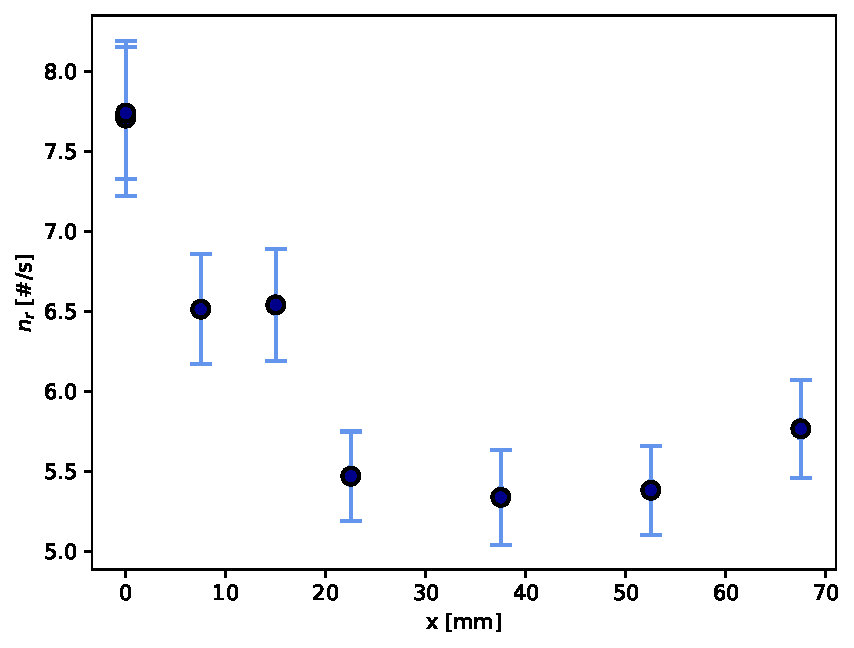
\includegraphics[width=0.5\linewidth]{../Graficas/Atenuacion_Pb2.pdf}
\end{figure}


\section{Flujo en la superficie}


\section{Eficiencia geométrica}


\subsection{Dependencia con la distancia}

\begin{center}
\begin{table}[H]
\caption{Medidas de coincidencias a una distancia $d$ entre los detectores.}
\label{Tab:distancia}
\footnotesize
\begin{tabular}{cccccccccccccccccccccc}
\toprule
$d_{\text{real}}$ (cm) & $N_1$  & $N_2$ & $N_{12}$ & $t$ [s] & $n_1$ [s$^{-1}$] & $n_2$  [s$^{-1}$] & $n_{acc}$ [s$^{-1}$] & $n_{r}$ [s$^{-1}$] \\
\midrule
\num{2.7950000000(0.2100000000)} & \num{10319.0000000000(101.5824788042)} & \num{4468.0000000000(66.8430998683)} & \num{301.0000000000(17.3493515729)} & \num{41.1600000000(0.1300000000)} & \num{250.7045675413(2.5919038702)} & \num{108.5519922255(1.6597784794)} & \num{0.7478539177(0.0169783229)} & \num{6.5650712523(0.4224836365)} \\
\num{6.0950000000(0.2100000000)} & \num{8569.0000000000(92.5688932633)} & \num{3684.0000000000(60.6959636220)} & \num{212.0000000000(14.5602197786)} & \num{35.7400000000(0.1300000000)} & \num{239.7593732513(2.7329442325)} & \num{103.0777839955(1.7391596504)} & \num{0.6791370071(0.0156922779)} & \num{5.2525921479(0.4082654631)} \\
\num{6.0950000000(0.2100000000)} & \num{16455.0000000000(128.2770439323)} & \num{7216.0000000000(84.9470423264)} & \num{408.0000000000(20.1990098767)} & \num{69.1100000000(0.1300000000)} & \num{238.0986832586(1.9093998095)} & \num{104.4132542324(1.2447501412)} & \num{0.6831708914(0.0149963837)} & \num{5.2204609998(0.2928684246)} \\
\num{11.0950000000(0.2100000000)} & \num{22589.0000000000(150.2963738751)} & \num{9313.0000000000(96.5038859321)} & \num{411.0000000000(20.2731349327)} & \num{80.6500000000(0.1300000000)} & \num{280.0867947923(1.9174711458)} & \num{115.4742715437(1.2109668395)} & \num{0.8887806551(0.0192571525)} & \num{4.2073135793(0.2522421291)} \\
\num{11.0950000000(0.2100000000)} & \num{24440.0000000000(156.3329779669)} & \num{9925.0000000000(99.6242942259)} & \num{430.0000000000(20.7364413533)} & \num{89.9100000000(0.1300000000)} & \num{271.8273829385(1.7826391098)} & \num{110.3881659437(1.1194811437)} & \num{0.8245793415(0.0178137531)} & \num{3.9579809966(0.2314257978)} \\
\num{16.3950000000(0.2100000000)} & \num{29857.0000000000(172.7917822120)} & \num{12252.0000000000(110.6887528162)} & \num{416.0000000000(20.3960780544)} & \num{113.4800000000(0.1300000000)} & \num{263.1036305957(1.5522072527)} & \num{107.9661614381(0.9832135908)} & \num{0.7806048233(0.0167362779)} & \num{2.8852393784(0.1805591813)} \\
\num{21.5950000000(0.2100000000)} & \num{37079.0000000000(192.5590818424)} & \num{15964.0000000000(126.3487237767)} & \num{406.0000000000(20.1494416796)} & \num{141.6800000000(0.1300000000)} & \num{261.7094861660(1.3801636594)} & \num{112.6764539808(0.8977623996)} & \num{0.8103438941(0.0172485076)} & \num{2.0552687541(0.1432842454)} \\
\num{26.2950000000(0.2100000000)} & \num{48584.0000000000(220.4177851263)} & \num{20692.0000000000(143.8471410908)} & \num{419.0000000000(20.4694894905)} & \num{190.6800000000(0.1300000000)} & \num{254.7933710929(1.1689357556)} & \num{108.5168869310(0.7580094256)} & \num{0.7598050570(0.0160767553)} & \num{1.4375937263(0.1085574472)} \\
\num{30.9950000000(0.2100000000)} & \num{37162.0000000000(192.7744796388)} & \num{16595.0000000000(128.8215820428)} & \num{313.0000000000(17.6918060130)} & \num{152.2400000000(0.1300000000)} & \num{244.1014188124(1.2832952513)} & \num{109.0055176038(0.8512785517)} & \num{0.7311988734(0.0155524141)} & \num{1.3247653936(0.1172591881)} \\
\num{36.0950000000(0.2100000000)} & \num{44041.0000000000(209.8594767934)} & \num{18297.0000000000(135.2664038111)} & \num{324.0000000000(18.0000000000)} & \num{172.8000000000(0.1300000000)} & \num{254.8668981481(1.2295074061)} & \num{105.8854166667(0.7868344241)} & \num{0.7415941781(0.0157292873)} & \num{1.1334058219(0.1053569869)} \\
\num{40.9950000000(0.2100000000)} & \num{53537.0000000000(231.3806387752)} & \num{23429.0000000000(153.0653455228)} & \num{338.0000000000(18.3847763109)} & \num{218.3000000000(0.1300000000)} & \num{245.2450755841(1.0699349806)} & \num{107.3247824095(0.7040765782)} & \num{0.7232976278(0.0152710543)} & \num{0.8250303612(0.0855962423)} \\
\num{50.9950000000(0.2100000000)} & \num{59969.0000000000(244.8856876177)} & \num{26718.0000000000(163.4564162093)} & \num{325.0000000000(18.0277563773)} & \num{243.6300000000(0.1300000000)} & \num{246.1478471453(1.0136990854)} & \num{109.6662972540(0.6734678292)} & \num{0.7417984993(0.0156291432)} & \num{0.5921915676(0.0756323487)} \\
\num{57.2950000000(0.2100000000)} & \num{44514.0000000000(210.9834116702)} & \num{19942.0000000000(141.2161463856)} & \num{210.0000000000(14.4913767462)} & \num{180.4000000000(0.1300000000)} & \num{246.7516629712(1.1829712455)} & \num{110.5432372506(0.7868373835)} & \num{0.7495644750(0.0158769298)} & \num{0.4145153476(0.0818874302)} \\
\bottomrule
\end{tabular}
\end{table}
\end{center}


\begin{figure}[h!] \centering
    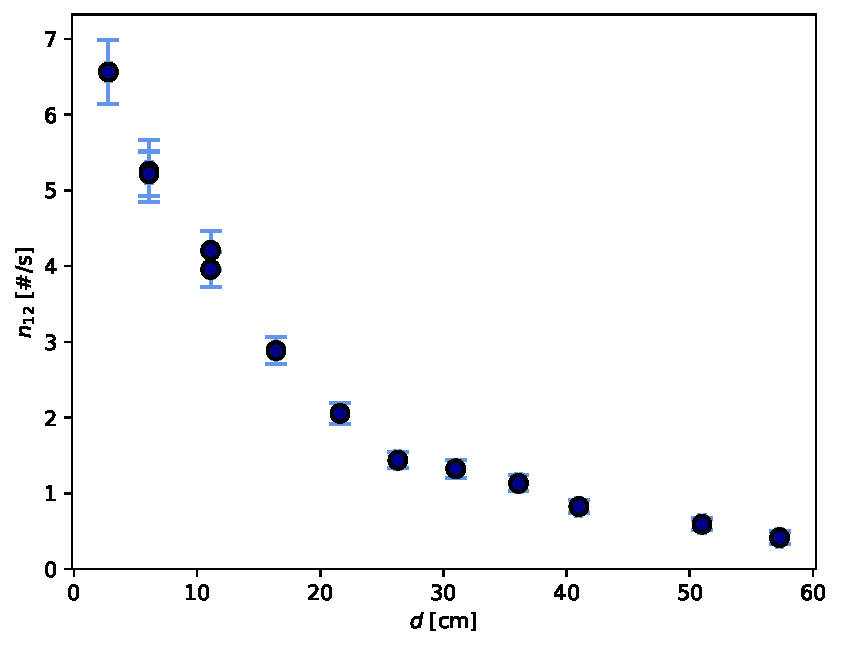
\includegraphics[width=0.5\linewidth]{../Graficas/Distancias.pdf}
\end{figure}


\subsection{Dependencia con el ángulo}

\begin{center}
\begin{table}[H]
\scriptsize
\caption{Medidas de coincidencias a una distancia $33.3$ cm entre los detectores a diferentes ángulos. Factor de cobertura al ángulo de $k=3$.}
\label{Tab:angulo}
\begin{tabular}{cccccccccccccccccccccc}
\toprule
$\theta$ ($^\circ$) & $N_1$  & $N_2$ & $N_{12}$ & $t$ [s] & $n_1$ [s$^{-1}$] & $n_2$  [s$^{-1}$] & $n_{acc}$ [s$^{-1}$] & $n_{r}$ [s$^{-1}$] \\
\midrule
\num{0.00} & \num{44041.0000000000(209.8594767934)} & \num{18297.0000000000(135.2664038111)} & \num{324.0000000000(18.0000000000)} & \num{172.8000000000(0.1300000000)} & \num{254.8668981481(1.2295074061)} & \num{105.8854166667(0.7868344241)} & \num{0.7415941781(0.0157292873)} & \num{1.1334058219(0.1053569869)} \\
\num{10.0000000000(0.8400000000)} & \num{55792.0000000000(236.2033022631)} & \num{25452.0000000000(159.5368296037)} & \num{399.0000000000(19.9749843554)} & \num{227.8300000000(0.1300000000)} & \num{244.8843435895(1.0461263694)} & \num{111.7148751262(0.7031404583)} & \num{0.7517765118(0.0158536022)} & \num{0.9995292864(0.0891023711)} \\
\num{25.0000000000(0.8400000000)} & \num{51215.0000000000(226.3073131828)} & \num{22894.0000000000(151.3076336475)} & \num{331.0000000000(18.1934053987)} & \num{210.6000000000(0.1300000000)} & \num{243.1861348528(1.0850181877)} & \num{108.7084520418(0.7215867426)} & \num{0.7264719499(0.0153462314)} & \num{0.8452279552(0.0877462853)} \\
\num{45.0000000000(0.8400000000)} & \num{65255.0000000000(255.4505823051)} & \num{27374.0000000000(165.4508990607)} & \num{316.0000000000(17.7763888346)} & \num{259.8700000000(0.1300000000)} & \num{251.1063223920(0.9909874155)} & \num{105.3372840266(0.6388449225)} & \num{0.7268695779(0.0153046083)} & \num{0.4891230338(0.0700987542)} \\
\num{60.0000000000(0.8400000000)} & \num{52123.0000000000(228.3046210658)} & \num{23612.0000000000(153.6619666671)} & \num{303.0000000000(17.4068951855)} & \num{219.3800000000(0.1300000000)} & \num{237.5923055885(1.0501617100)} & \num{107.6305953141(0.7033352378)} & \num{0.7027240915(0.0148373861)} & \num{0.6784410101(0.0807253596)} \\
\num{67.0000000000(0.8400000000)} & \num{56803.0000000000(238.3337995333)} & \num{27445.0000000000(165.6653252796)} & \num{315.0000000000(17.7482393493)} & \num{218.2500000000(0.1300000000)} & \num{260.2657502864(1.1029711076)} & \num{125.7502863688(0.7627488804)} & \num{0.8993789775(0.0189496636)} & \num{0.5439199916(0.0835037875)} \\
\num{77.0000000000(0.8400000000)} & \num{68655.0000000000(262.0209915255)} & \num{29397.0000000000(171.4555335940)} & \num{301.0000000000(17.3493515729)} & \num{267.5000000000(0.1300000000)} & \num{256.6542056075(0.9874271286)} & \num{109.8953271028(0.6431764675)} & \num{0.7750760897(0.0163044246)} & \num{0.3501575552(0.0668776062)} \\
\num{90.0000000000(0.8400000000)} & \num{72191.0000000000(268.6838290631)} & \num{30162.0000000000(173.6721048413)} & \num{292.0000000000(17.0880074906)} & \num{280.0100000000(0.1300000000)} & \num{257.8157922931(0.9669875466)} & \num{107.7175815149(0.6222482657)} & \num{0.7631551487(0.0160463202)} & \num{0.2796647506(0.0631026352)} \\
\bottomrule
\end{tabular}
\end{table}
\end{center}


\begin{figure}[h!] \centering
    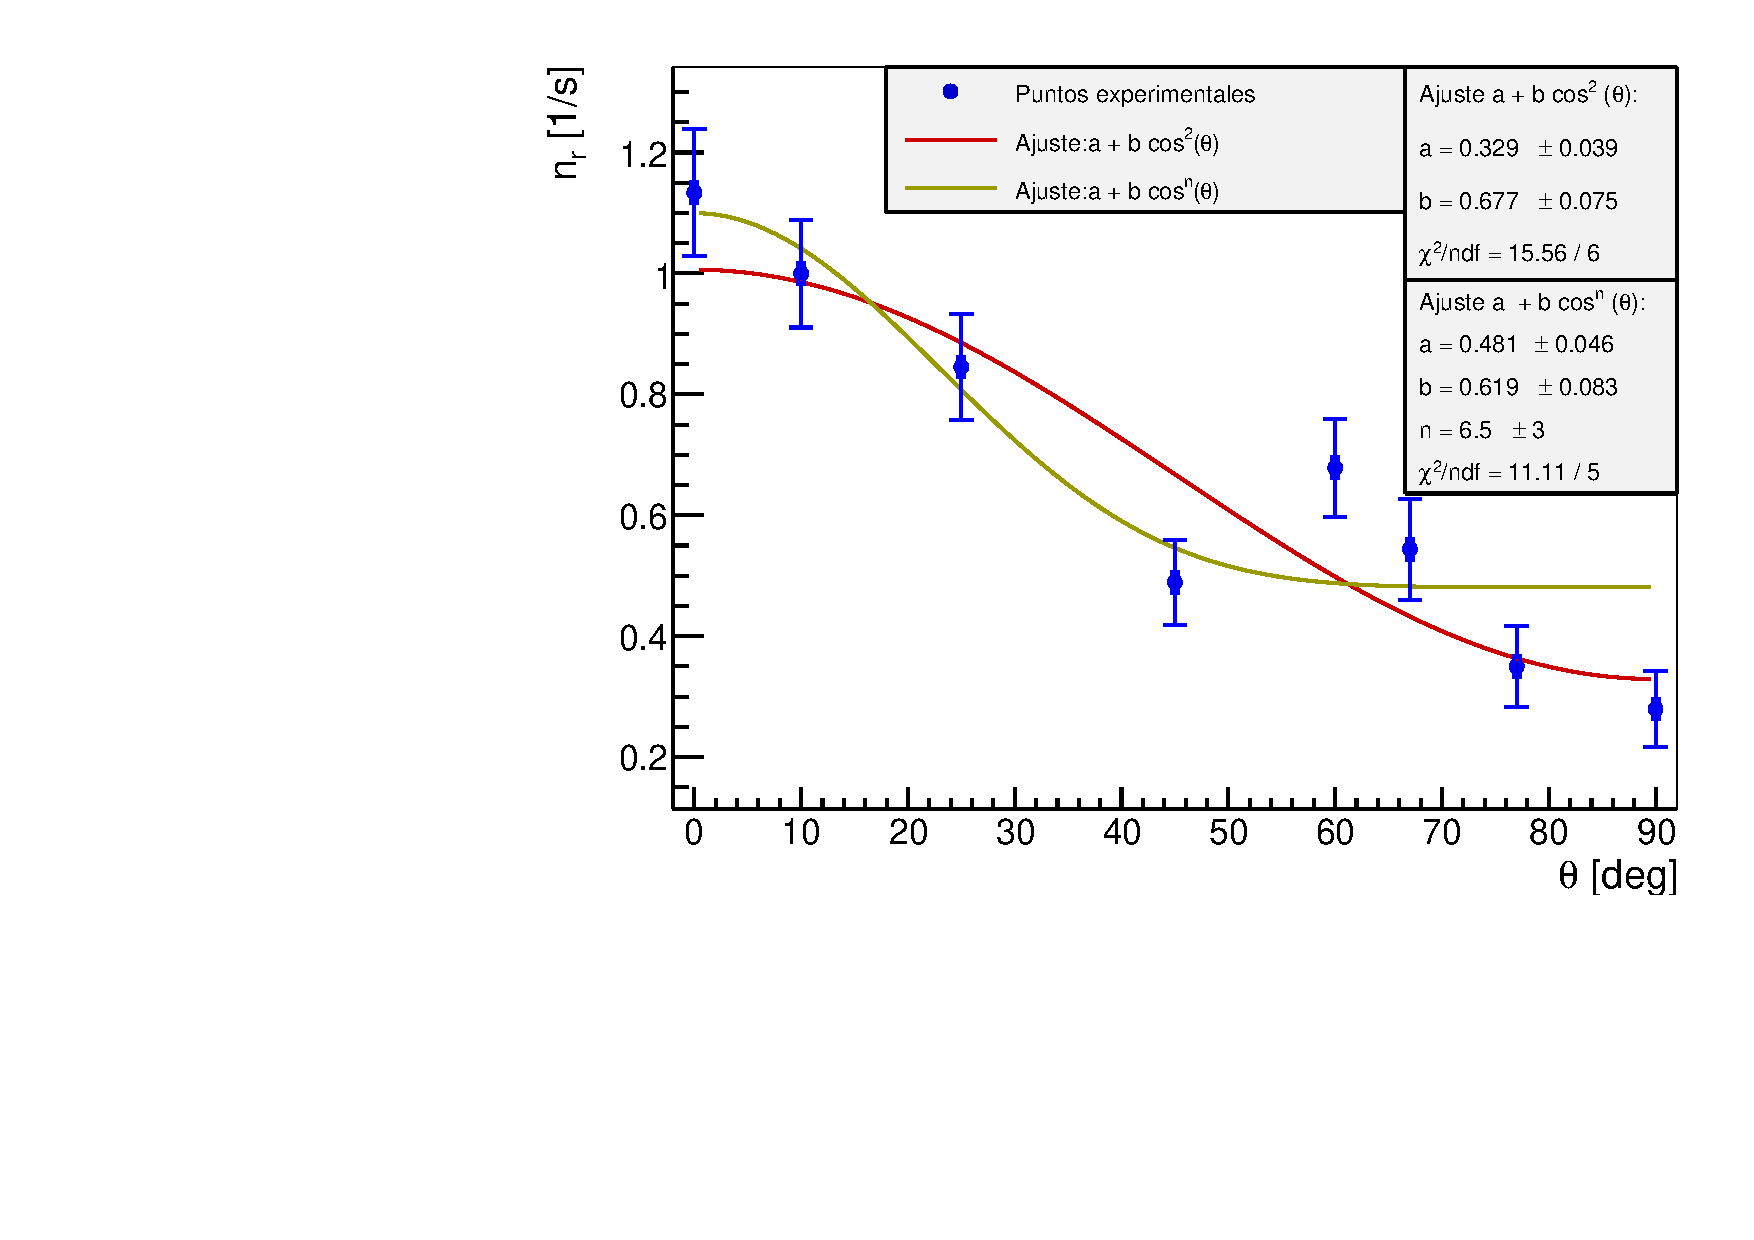
\includegraphics[width=0.5\linewidth]{../Graficas/Angulos.pdf}
\end{figure}

\subsection{Montecarlo}


\appendix

\section{Tablas}



\printbibliography
\addcontentsline{toc}{section}{Bibliografía}


\end{document}